\section{Introduction}
\label{sec:intro}
%设计了一套方法,使得之前的baseline都可以在异构模型之间做merging,这是异构模型无需额外开销的第一次merging尝试。
%利用异构特性融合后的模型可以超越原模型,并且在多个任务上达到了vlm-7B的sota
%merging方法众多各有所长,我们设计了一套无监督自动的模型选择方法,对于每个任务无需label就能adaptive的选择最优的融合模型。


% model-merging的背景,为什么流行。 首先是llm流行,但是缺点,微调容易遗忘,训练成本高。   现在的情况,llm很多。各种场景拿不到数据。

%现有的方法怎么做的。1.只能在同构模型merge,没有利用异构的优点 2. 这些方法都有一个关键性的超参数需要调节。需要知道下游任务的答案。
% Multimodal Large Language Models (MLLMs) have gained extensive popularity in real-world applications. Fine-tuning with labeled data is essential for adapting them to specific tasks. However, fine-tuning often leads to catastrophic forgetting, reduces the pre-trained model's capabilities, and requires significant amounts of training data and computational resources.
% As a result, there is a growing interest in developing efficient and lightweight methods to optimize MLLMs. The availability of numerous open-source MLLMs provides an opportunity to combine them into a more powerful and versatile model without the need of resource-intensive training process, which can be achieved via model merging techniques.
%改为:

\begin{figure*}
    \centering
    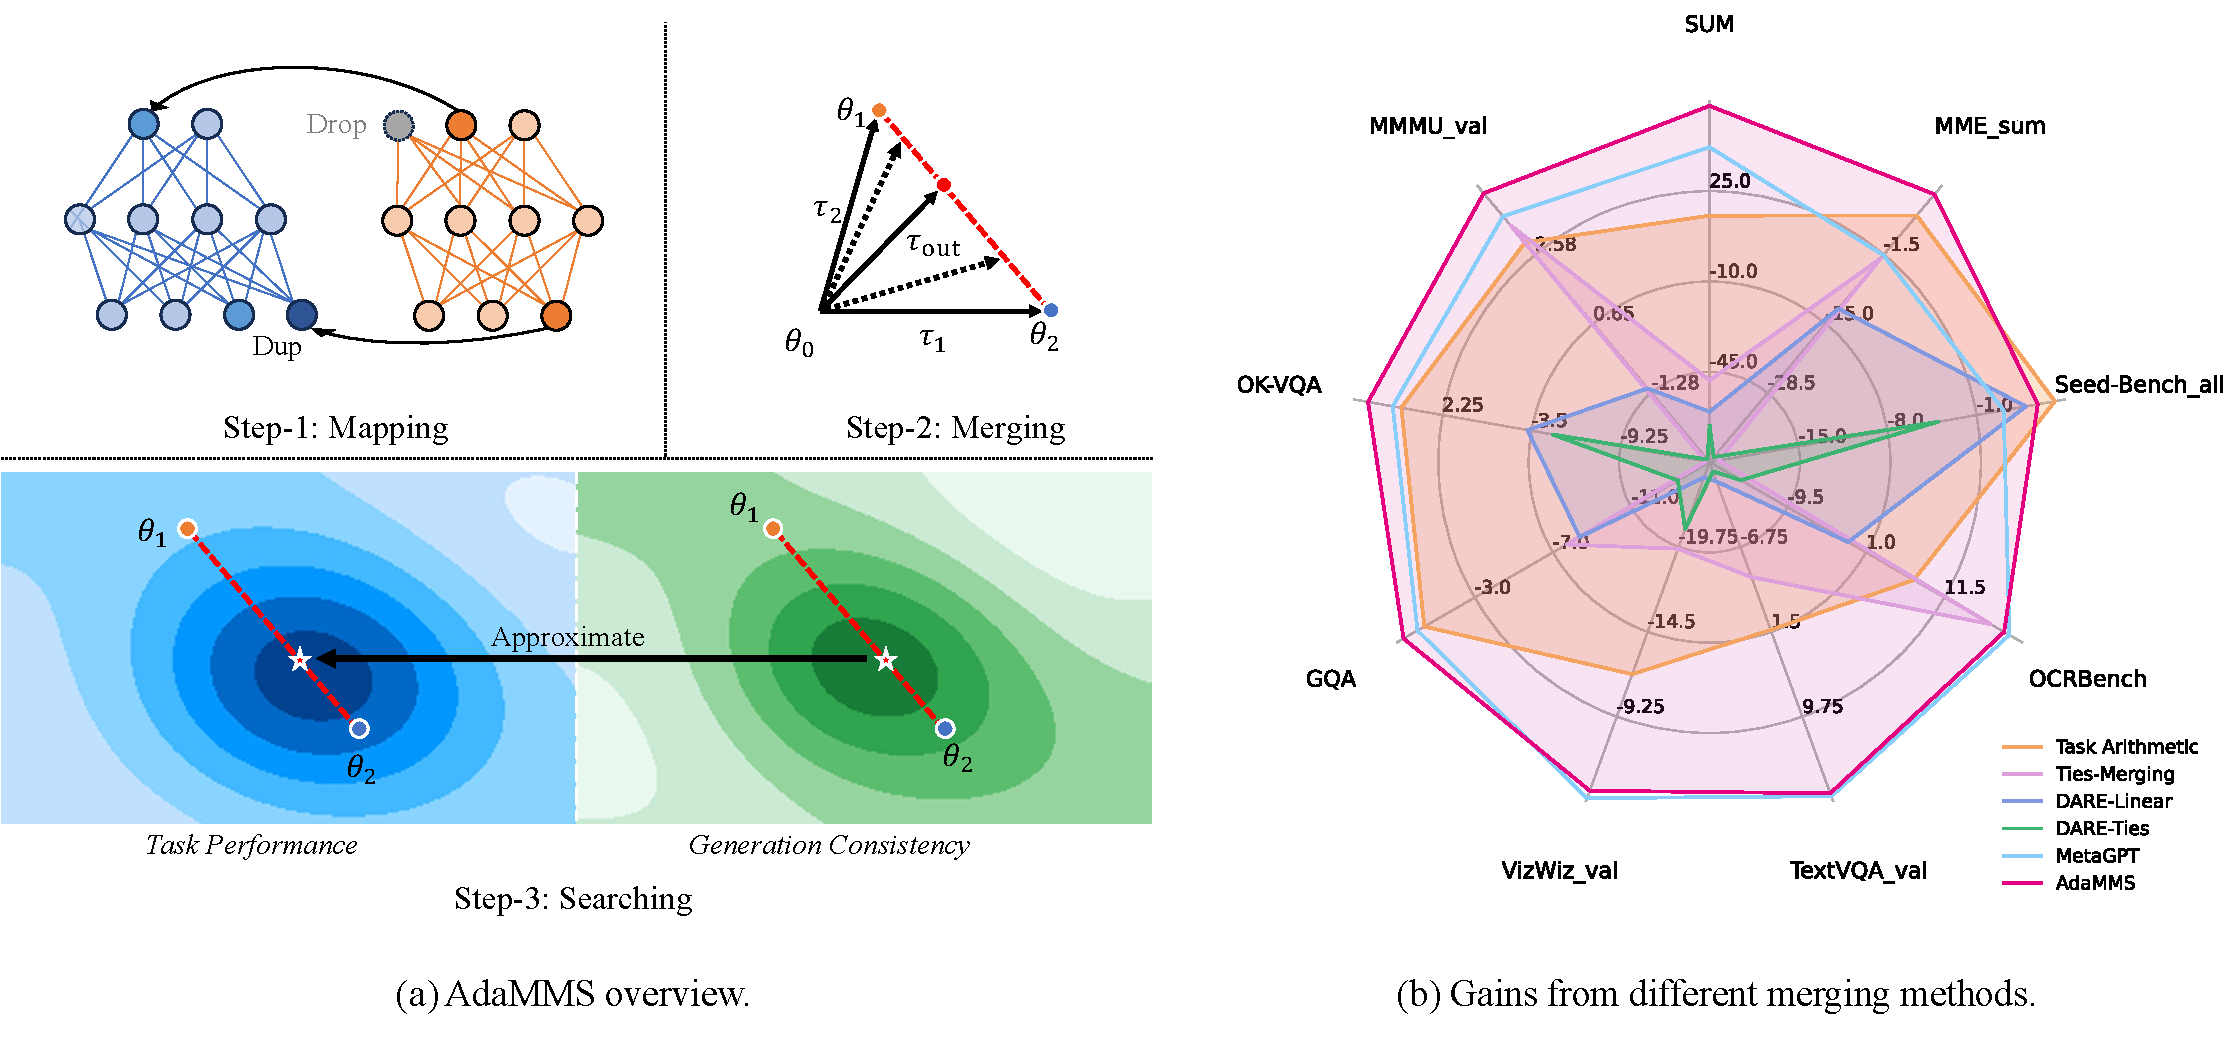
\includegraphics[width=0.9\linewidth, bb=0 0 1074 498]{figure/head.pdf}
    \caption{(a) Illustration of three steps in AdaMMS: Step-1, mapping MLLMs with different model architecture; Step-2, merging MLLMs with linear interpolation; Step-3, searching for optimal merging hyper-parameter by approximate task performance through generation consistency without labeled data. (b) The gain performance of AdaMMS on a broad range of multimodal tasks in comparison with existing merging approaches. Gain refers to the improvement obtained by subtracting the average result from the result of the fused model on a certain task. The result here is the average of the gains from the two MLLM pairs merging. }
    \label{fig:figure1}
\end{figure*}

% \begin{figure*}
%     \centering
   
%     \begin{subfigure}[a]{0.45\textwidth}
        
%         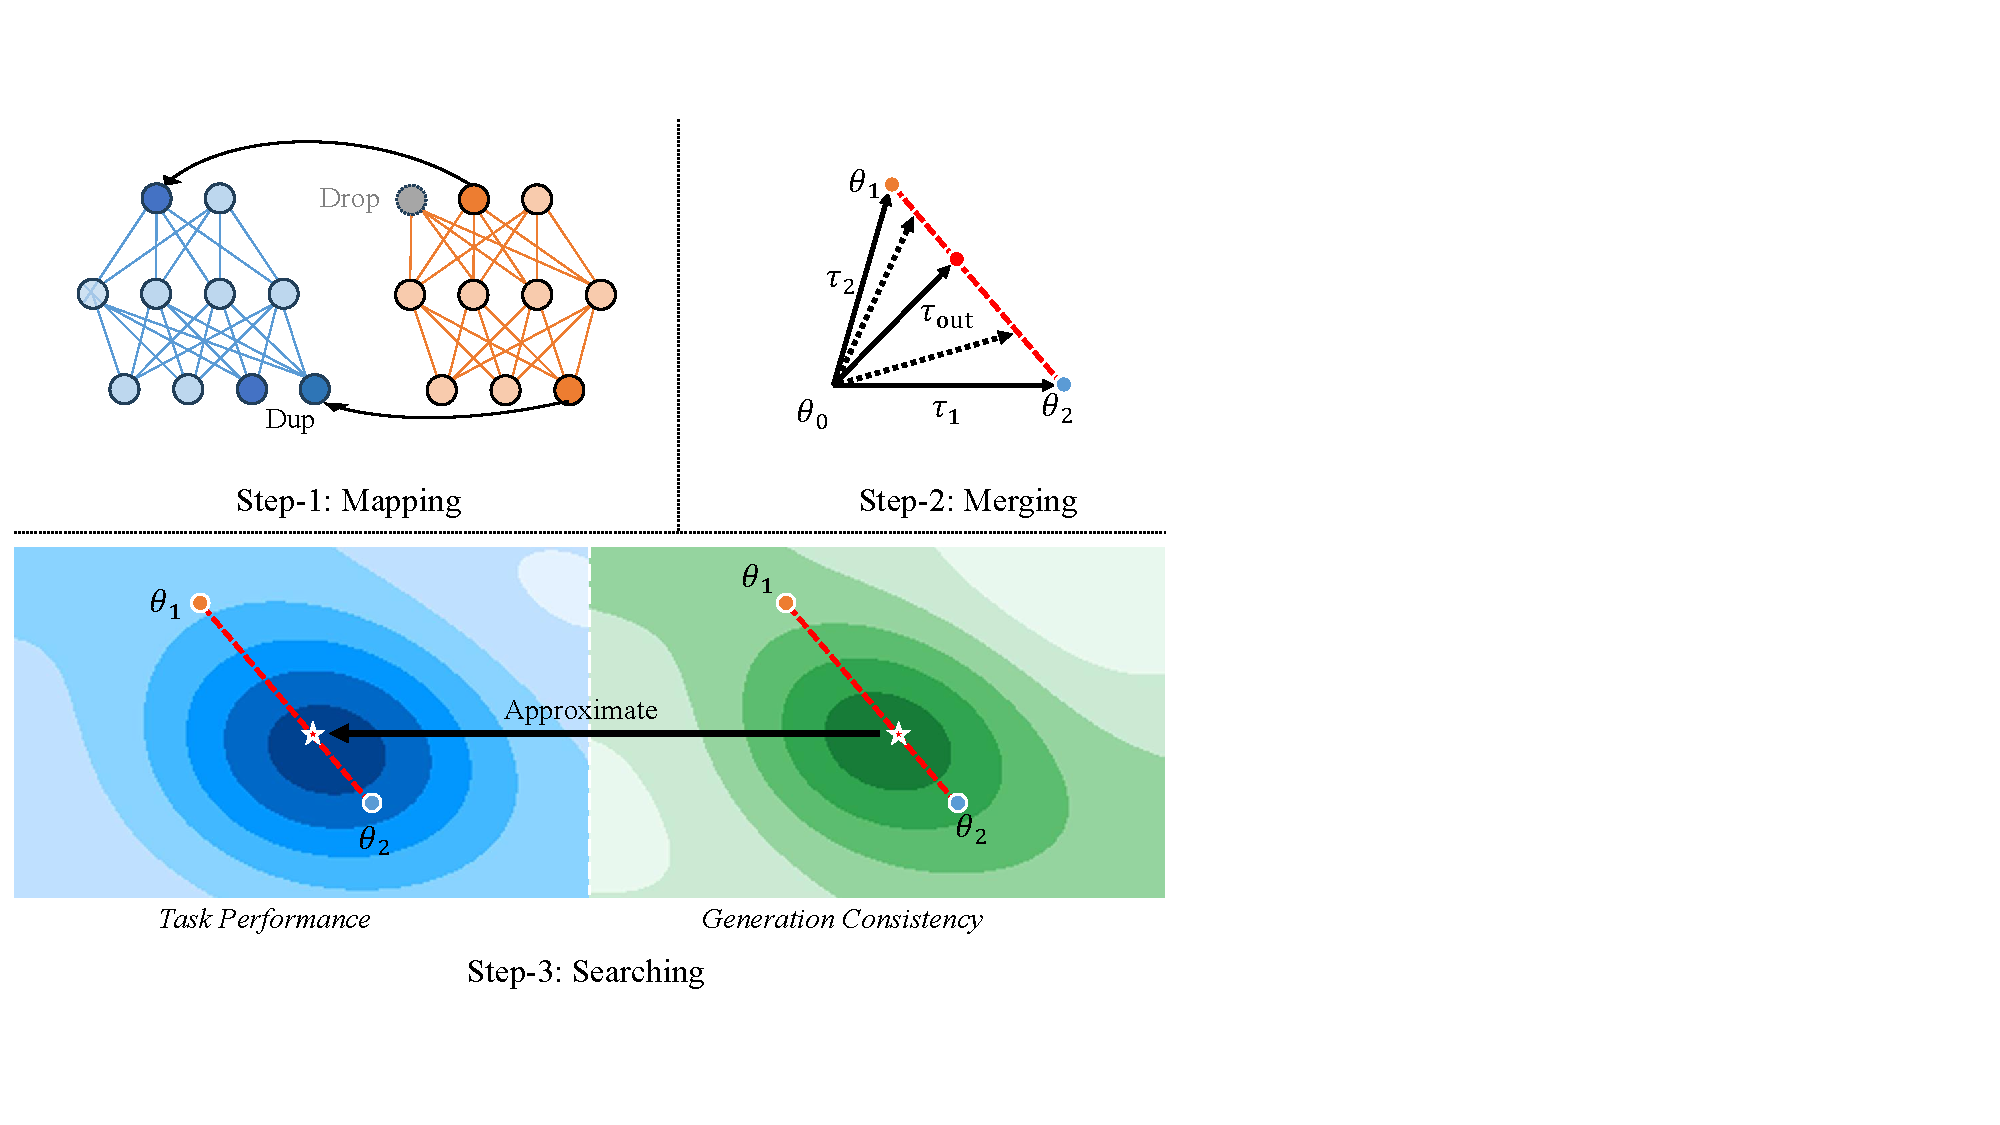
\includegraphics[width=\textwidth]{figure/crop_head_figure.pdf}
%         \caption{AdaMMS overview.}
%     \end{subfigure}
%     \begin{subfigure}[b]{0.4\textwidth}
       
%         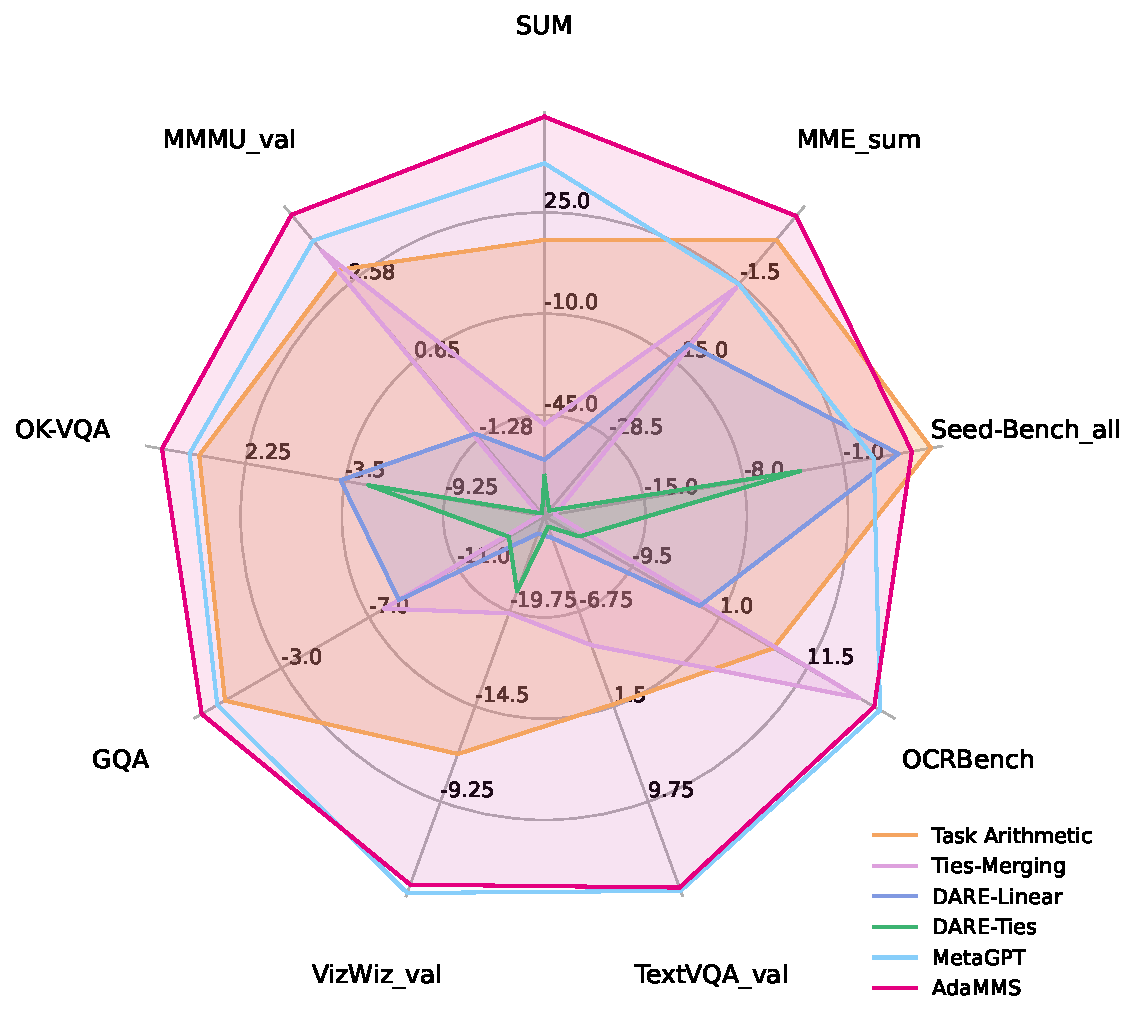
\includegraphics[width=\textwidth]{figure/radar_compare.pdf}
%         \caption{Performance}
%     \end{subfigure}
%     \caption{(a) Illustration of three steps in AdaMMS: (a) mapping MLLMs with different model architecture, (b) merging MLLMs with linear interpolation, and (c) searching for optimal merging hyper-parameter by approximate task performance through generation consistency without labeled data. (b) The performance of our \our on a broad range of multimodal tasks in comparison with existing merging approaches. }
%     \label{fig:figure1}
% \end{figure*}


% \begin{figure*}[t]
%     \centering
%     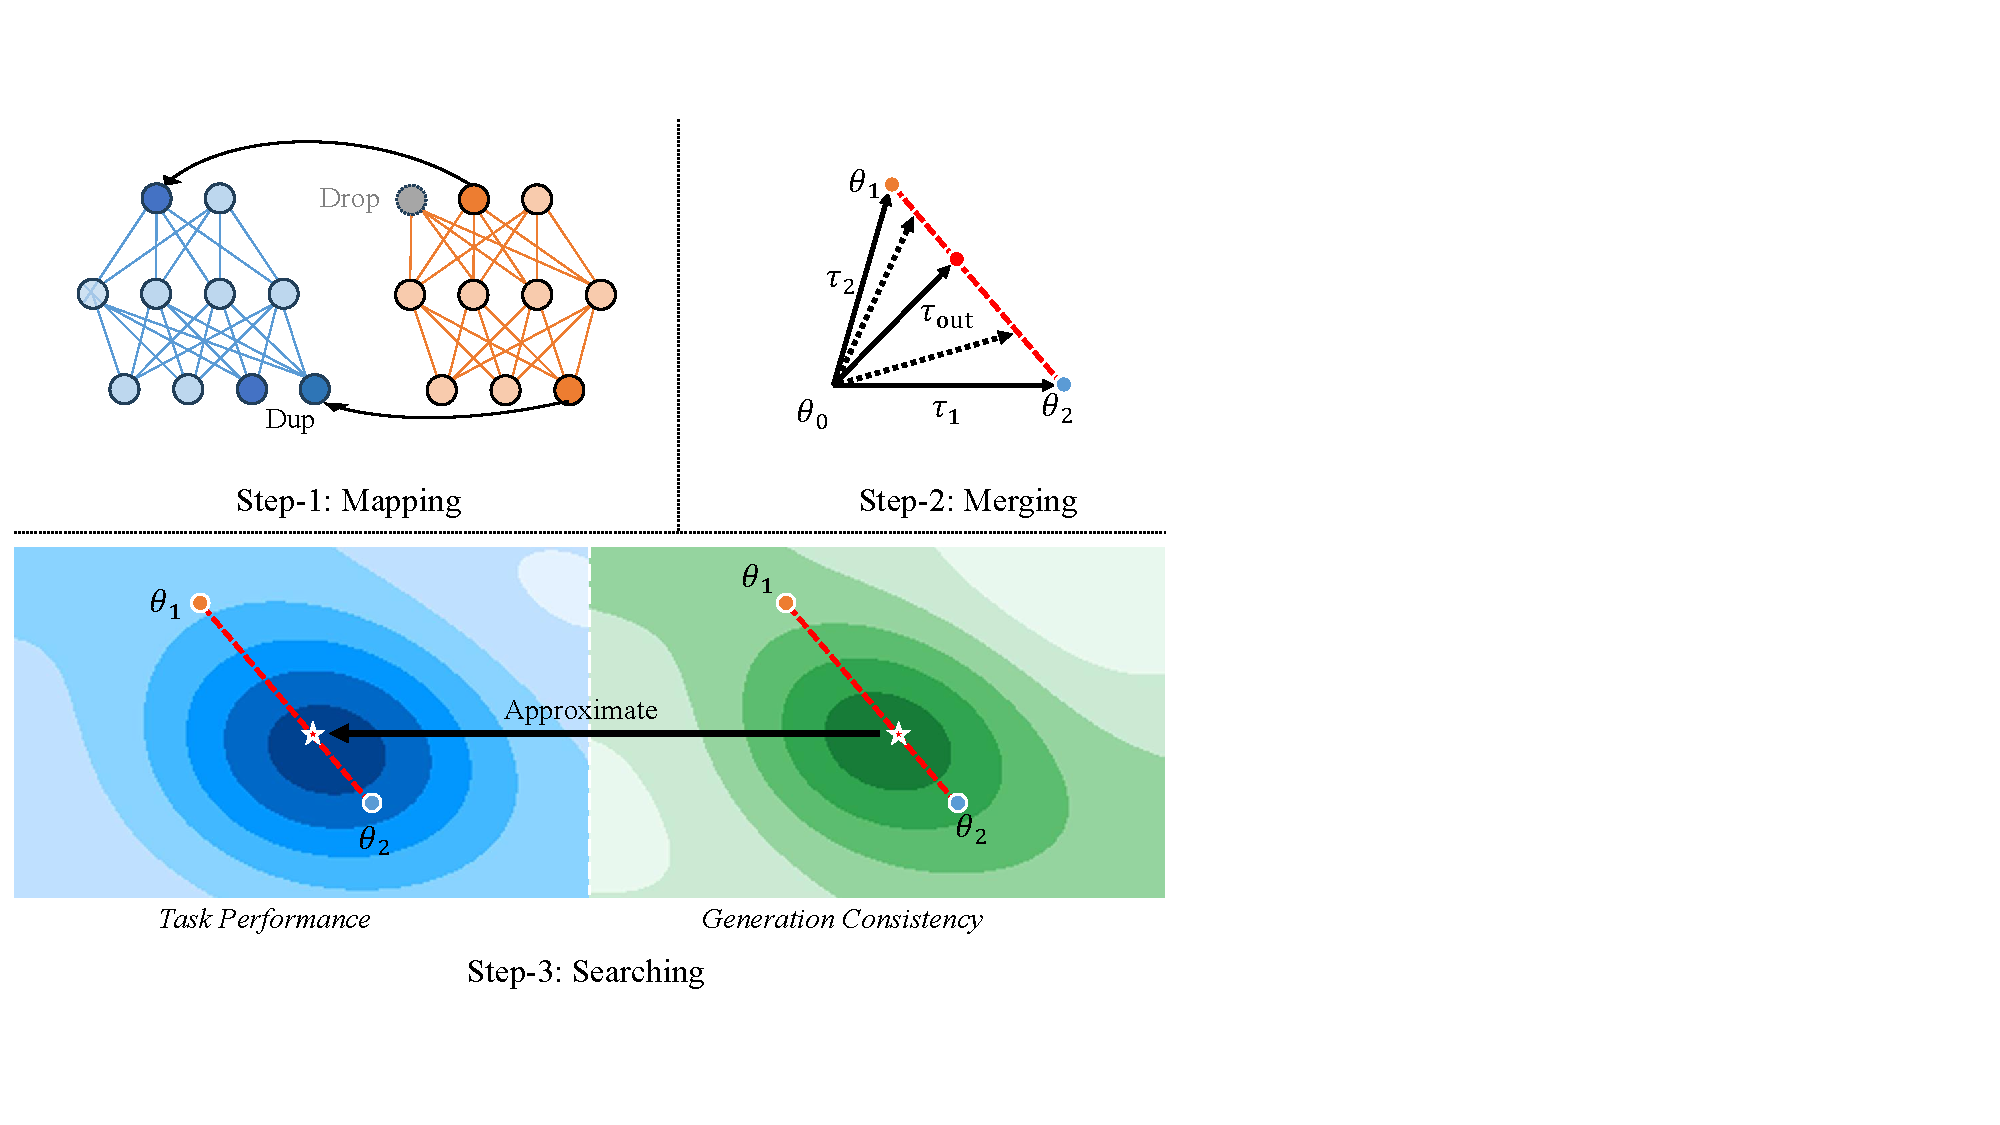
\includegraphics[width=1.0\textwidth]{figure/crop_head_figure.pdf}
%     \caption{Illustration of three steps in AdammS: (a) mapping MLLMs with different model architecture, (b) merging MLLMs with linear interpolation, and (c) searching for optimal merging hyper-parameter by approximate task performance through generation consistency without labeled data.}
%     \label{fig:figure1}
% \end{figure*}

Model merging~\cite{task-arithmetic} has gained increasing popularity in the field of large language models~(LLMs)~\cite{task-arithmetic, ties, dare, metagpt}. This approach typically involves combining the parameters of two models with the same architecture, creating a new model without requiring additional training~\cite{task-arithmetic}. It has proven to be an efficient method for developing models that integrate the abilities of multiple existing models~\cite{ties, dare, metagpt}, avoiding the need for extensive data and computational resources, and has been widely adopted in building powerful LLMs~\cite{goddard2024mergekit,open-llm-leaderboard-v2}.

% Model merging techniques \cite{task-arithmetic}, which fuses the parameters of various models to create a unified one, have demonstrated promising results in combining different capabilities of various large language models (LLMs)~\cite{task-arithmetic, ties, dare, metagpt}. 
% Recently model merging gains popularity since it is an efficient paradigm of creating a model with the abilities from multiple existing models that requires no intensive data and computation cost, compared with paradigms like supervised fine-tuning. And various model merging strategies \cite{task-arithmetic, ties, dare, metagpt} have been proposed to improve the performance of the generated LLM.

Despite its popularity with LLMs, model merging has yet to be widely adopted for multimodal large language models~(MLLMs). Some recent studies have explored the application of model merging to MLLMs~\cite{sung2023empirical,modelcompose} but either prioritize extending multimodal capabilities over enhancing the performance of existing models~\cite{modelcompose} or still require additional training after merging~\cite{sung2023empirical}. The primary obstacle in applying model merging to MLLMs lies in the heterogeneous nature of these models~\cite{llava1.5, qwen2-vl, cogvlm2, llava-onevison, mplugowl2}.  This heterogeneity arises from modifications to the transformer architectures~\cite{attention} within their language models~\cite{cogvlm2,mplugowl2}, as well as differences in their choice of modality-specific encoders and tokenizers~\cite{qwen2-vl, cogvlm2}. Consequently, a significant challenge in merging MLLMs is that the process cannot be directly applied to models with different architectures, as their weights are not isomorphic.

Recent efforts like FuseLLM~\cite{fusellm} and FuseChat~\cite{fusechat} have explored fusing the capabilities of heterogeneous LLMs by merging their generative distributions. Theoretically, these methods could also be applied to MLLMs. However, they rely on supervised continued training, which incurs significant computational costs and fails to address scenarios where labeled data is unavailable. For example, FuseLLM requires a training dataset with a total of 1.8 billion tokens and 33 hours of training time. This underscores the need for an unsupervised model merging technique to effectively integrate heterogeneous MLLMs.

% These factors introduce two major challenges to model merging for MLLMs: (1)  the merging process cannot be directly applied to MLLMs with differing architectures, as their model weights are not isomorphic, and (2) using existing merging strategies on MLLM parameters often leads to suboptimal performance. Since these challenges are uncommon when merging LLMs, most current model merging methods have not been designed to address them effectively~\cite{task-arithmetic, ties, dare, metagpt}. To fuse heterogeneous LLMs, FuseLLM \cite{fusellm} and FuseChat \cite{fusechat} leverage the knowledge distillation process to enable the fusion among LLMs with different architecture. But their methods require supervised continue training, which brings the need of labeled data.

% As a result, there is a growing interest in applying such an efficient and lightweight paradigm to multimodal large language models (MLLMs) \cite{sung2023empirical,sundar2023multimodal,modelcompose}. 
% %[TODO: more model merging on MLLMs?]
% However, current methods fall short on obtaining satisfying results in merging MLLMs. The main obstacle lies in the heterogeneous nature of MLLMs \cite{llava1.5, qwen2-vl, cogvlm2, llava-onevison, mplugowl2}, due to modifications made to the transformer \cite{attention} architectures within their language models, as well as differences in their choice of modality-specific encoders and tokenizers. Consequently, the heterogeneous nature brings two primary challenges to model merging on MLLMs: (1) we cannot directly apply the model merging process to MLLMs with different architectures, as their model weights are not isomorphic, and (2) applying current merging strategies to MLLM parameters often resulting in suboptimal performance, according to our experiments. Although these challenges are common for MLLMs, they do not typically occur when merging LLMs. Thus, few existing model merging methods have been designed to address these challenges. % , which calls for further investigation on model merging for heterogeneous MLLMs.

% TODO: 这个放到4.Experiments里边去讲
% The performance of the merged model degrades significantly when the merged parameters deviate too much from the original parameters in the base architecture, even if they are similar with the weights of another model.

% Pioneering works on fusing heterogeneous LLMs and MLLMs mainly fall into two categories. On one hand, FuseLLM \cite{fusellm} and FuseChat \cite{fusechat} leverage the knowledge distillation process to enable the fusion among LLMs with different architecture. But their methods require supervised continue training, which brings the need of labeled data.
% %TODO: "That is hard to find in some scenarios?"
% On the other hand, X-InstructBLIP \cite{xinstructblip} and DAMC \cite{modelcompose} leverage modality projectors and the model merging technique for multimodal fusion in MLLMs with different modality encoders, but they still focus on models with the identical language model architecture, and they also need labeled data on validation set for hyper-parameter tuning.
% % TODO:tuning or selection?
% Hence, there remains a necessity for an unsupervised model merging technique to integrate heterogeneous MLLMs effectively.

In this work, we address the challenges of merging heterogeneous MLLMs by introducing a novel model merging strategy named \ours
% ~\footnote{\textbf{Ada}ptive \textbf{M}apping, \textbf{M}erging, and \textbf{S}earching}
, as illustrated in Figure~\ref{fig:figure1}.
First, to enable model merging across heterogeneous MLLMs with differing architectures, we design a parameter mapping framework. Specifically, we focus on the scenario where MLLMs have different language model architectures due to variations in transformer block duplications \cite{cogvlm, cogvlm2, mplugowl2}. This mapping aligns corresponding components across models, enabling merging operations even with structural differences. Next, we apply adaptive linear interpolation on the mapped parameters during merging. By adjusting the interpolation coefficient, \ours optimizes performance adaptively across different tasks. This coefficient adjustment is then optimized through an unsupervised procedure in the following step. Finally, we introduce an \textbf{unsupervised} hyperparameter selection method to determine the interpolation coefficient for each task. This approach leverages response consistency across candidate models as a performance estimate, based on our novel insight that model performance correlates with generation consistency. In addition to strong empirical support, we provide a theoretical analysis to explain this insight.

% In this work, we tackle the aforementioned challenges by proposing a novel model merging strategy named \ours~\footnote{\textbf{Ada}ptive \textbf{M}apping, \textbf{M}erging and \textbf{S}earching}, as shown in the Figure~\ref{fig:figure1}.
% First, to enable model merging methods being performed on heterogeneous MLLMs with architecture difference, we design a mapping between the parameters of different MLLMs. We focus on the heterogeneous scenario where the MLLMs have different language model architecuture due to duplications on transformer block components \cite{cogvlm, cogvlm2, mplugowl2}.
% % For example, CogVLM \cite{cogvlm} adapts visual experts by duplicating query, key and value weights in attention head. mPLUG-Owl2 \cite{mplugowl2}, on the other hand, is designed to duplicate key, value, and layer norm weights instead. 
% % In this case, the principle of our mapping is connecting the relevant components of parameters with respect to their function in the model, which will facilitate the merging process later. 
% And the mapping connects the corresponding components of parameters in different models, which allows for merging operations on heterogeneous model structures.
% % Second, to adapt the asymmetry of the parameter space in merging MLLMs, we apply linear interpolation on merging strategy to actively leverage the heterogeneous property of MLLMs for better adaptation on various downstream tasks. 
% Second, we adapt linear interpolation on mapped model parameters in the merging step. Adjusting the coefficient of linear interpolation enables \ours to adaptively optimize performance across various tasks, and it allows us to perform the unsupervised coefficient optimization in the following step.
% Third, we design an \textbf{unsupervised} hyper-parameter selection method to choose linear interpolation coefficient on each task using the response differences from candidate models. It is based on our novel discovery that the model performance can be estimated by the generation consistency. Apart from strong experimental evidence, we also analyze the rationality of this discovery in theory.

% Specifically, we notice that when applying model merging techniques, several merging-related hyper-parameters have to be chosen. Previous works mostly adapts a supervised search on a validation dataset to determine the best combination of hyper-parameters. The supervised search requires labeled data for validation, which is hard to obtained in some scenario and have potential trouble accommodating data distribution shift between the validation-time tasks and the test-time tasks. 
% Therefore, we proposed a unsupervised performance estimation metric via comparing the difference on generation outputs. The effectiveness of this metric is based on a novel discovery on the landscape of the parameter space.  we noticed that in a variation process of a hyper-parameter, the difference in the performance of the merged model can be approximated by the difference of generated results, regardless of the ground truth.  This discovery allows us to develop an unsupervised hyper-parameters selection method on downstream tasks with limited unlabeled data needed, and improve the out-of-distribution data robustness during model merging at the same time.
%OOD

%---

% Model merging technique involves combining parameters from multiple distinct models with varying capabilities to create an universal model without the need for any training data or intensive computation resources.
% Current efforts like Task-Arithmetic, Ties-Merging and DARE mainly focus on improving the performance of the merged model for LLMs by optimizing merging strategies on model parameters. They have demonstrated promising results on integrating the abilities in different fine-tuned checkpoints of LLMs.
% However, current methods fall short on obtaining satisfying results in merging MLLMs. The main obstacle here is that MLLMs often contains more heterogeneous property, while LLMs are often homogeneous. The heterogeneous property of MLLMs includes two major gaps: (1) \textbf{representation gap}, MLLMs often use modality-specific encoders or tokenizers to extract representation features from multimodal inputs, and merging these models with different encoders or tokenizers has to deal with the representation gap caused by this difference between the models; (2) \textbf{architecture gap}, unlike LLMs, which commonly follow the standard decoder-only transformer architecture, MLLMs sometimes adapt structural modification in their language model. 
% For example, CogVLM adapts visual experts by duplicating query, key and value matrix in attention head. The mPLUG-Owl2 model, on the other hand, is designed to duplicate key, value matrix and layer norm instead. % TODO: 这个 For example 后边的例子是不是太繁琐了?
% % These structural modification v asymmetry in the parameter space, leading to architecture gap.

% There are pioneering works on fusing heterogeneous LLMs. FuseLLM and FuseChat leverage the knowledge distillation process to enable the fusion among LLMs with different architecture. But their method requires additional training process, which brings data and computational complexity to the model merging method. More importantly, previous paradigms do not actively leverage the heterogeneous property of MLLMs, resulting in suboptimal integration of multimodal capabilities and limited model effectiveness.

% Moreover, we notice that when applying current model merging methods, several merging-related hyper-parameters have to be specified. Previous works mostly applies supervised searching on a validation dataset to determine the best combination of hyper-parameters. The supervised searching requires labeled data for validation, and is hard to accommodate data distribution shift between the validation-time data and the test-time data. 
% In this work, we proposed a \textit{unsupervised} performance estimation metric based on our novel discovery on the landscape of the parameter space. As shown in the Figure 1 (TODO), we noticed that in a variation process of a hyper-parameter, the difference in the performance of the merged model can be approximated by the difference of generated results, regardless of the ground truth.  This discovery allows us to develop an unsupervised hyper-parameters selection method on downstream tasks with limited unlabeled data needed, and improve the out-of-distribution data robustness during model merging at the same time.
% %OOD

% Therefore, to address the challenges in merging heterogeneous MLLMs, we propose Mms-Merging (mapping, merging, searching) method, a model merging method in three steps: First, we design a mapping between the parameters of different MLLMs to allow model merging operation performing on MLLMs with different architecture. Second, we apply linear interpolation on merging strategy to actively leverage the heterogeneous property of MLLMs on the adaptation to various downstream tasks. Third, we adaptively select the optimal hyper-parameters, including linear interpolation coefficient, for each task using the response differences from candidate models.

%% Other methods propose converting multiple heterogeneous models into homogeneous models through additional training before merging. 之前异构融合方法是需要先训练转到同一结构上再merging。 Knowledge Fusion of Large Language Models/ fusechat:knowledge of chat models / 还有Model Merging in LLMs, MLLMs, and Beyond: Methods, Theories, Applications and Opportunities 综述中2.2.2 Architecture Transformation

%怎么引出alpha需要调节的问题呢?万一别人不知道alpha 超参是干嘛的
% Homogeneous models exhibit minor variations and are closely positioned within the landscape, making their integration straightforward and leading to marginal improvements. In contrast, heterogeneous models differ significantly, with each potentially settling at distinct local optima. Merging these models poses substantial challenges but large improvements, due to the likelihood of surpassing local optima.


% Furthermore, former merging methods requires a effortlessly searching and 
% task-dependent hyperparameter, which is determined based on the label of the test set. But in some real-world application, we lack labeled data for certain tasks.


%In general, these methods involve processing task vectors derived by subtracting two target models from their original pre-trained models. Simple linear weighting often yields satisfactory results. Some methods involve parameter reduction to minimize interference between task vectors. 





% Our research suggests that existing multi-modal models, despite different structures, can be treated as meeting the aforementioned assumption if they stem from the same pre-trained large language model. By establishing specific rules and mappings, we can compute task vectors among the extract parameters, and consider those as homogeneous fusion operations. 
% Based on this assumption, we introduce a novel hypothesis that the optimization space for parameter linear interpolation exhibits smooth characteristics. Consequently, when interpolating with varying coefficients, we consider the similar inference performance between two coefficient as optimal values. 
% This obviates the need for labeled data during searching the coefficient, enabling automatic determination of optimal values for each task.

Extensive experiments have demonstrated the effectiveness of our proposed \ours in merging MLLMs. Our main experiments are conducted on two pairs of heterogeneous MLLMs, one of them is based on Qwen \cite{qwen2} architecture, another pair is based on LLaMA \cite{llama} architecture. Both experiments shows that our model can effectively combine the capabilities of heterogeneous MLLMs by enabling model merging on models with different architecture. The experiments also demonstrated that the merging strategy of \ours, accompanied with our unsupervised hyper-parameter selection method, outperforms previous model merging methods on various vision-language tasks. We also conducted experiments to show that the unsupervised hyper-parameter selection method can be performed with fewer unlabeled data without harming its performance, which shows the robustness of the method and further decrease the data requirements of \ours.

% By leveraging the fusion of Qwen-VL-7B and LLaVA-one-vision, we have achieved a new state-of-the-art at the 7B level. We obtained the best results in most tasks, attaining the highest overall performance. Significant improvements were also made through the fusion of other model pairs, including combinations among Qwen2-VL-7B \cite{qwen2-vl}, LLaVA-one-vision-QWEN \cite{llava-onevison}, LLaVA-1.5V-7B \cite{llava1.5}, Cogvlm-Chat \cite{cogvlm}, ShareGPT4V \cite{sharegpt4v}, and Mplug-owl2 \cite{mplugowl2}. Moreover, our approach exhibits great robustness and scalability, achieving results comparable to the full dataset with only 100 samples.
% TODO: 写完Experiment后改进这一段

Our main contributions are as follows:

\begin{itemize}
    % \item We propose a model merging strategy named \ours to tackle the heterogeneous challenges when merging MLLMs. By defining a mapping on parameters of different models, \ours enables model merging methods to be performed on MLLMs with architectural differences. The merging and searching steps of \ours further improve the performance on heterogeneous model merging.
    % By incorporating linear interpolation into model merging process, AdammS allows for the adaptive weighting of individual models, tailoring their contributions based on their relevance to specific downstream tasks.

    % \item We discovered a performance estimation metric on downstream tasks for model parameters that \textit{requires no labeled data}, through comparing relative differences of generated responses. We use empirical experiment results and theoretical analysis to showcase the effectiveness of the metric.

    % \item We proposed an \textit{unsupervised} hyper-parameter selection method based on the discovery that the model performance can be estimated by generation consistency, which is measured by the difference of generated responses. The unsupervised method gets rid of the need of labeled data in previous works. We further demonstrated that this method can be effectively applied to a small subset of the targeting data without compromising its performance.

    % \item We conducted extensive experiments on various model pairs, and main results on Qwen-based and LLaVA-based heterogeneous MLLM pairs both show that our model merging strategy can combine the abilities from heterogeneous MLLMs effectively, where \ours outperforms baseline strategies on various vision-language tasks and overall performance.

    \item We introduce a novel model-merging strategy, \ours, designed to address the challenges of merging heterogeneous MLLMs. By defining a parameter mapping between different models, \ours facilitates model merging techniques even when architectural differences exist.

    \item We propose an \textit{unsupervised} hyperparameter selection method inspired by the observation that model performance can be effectively estimated through generation consistency—measured by the variation in generated responses. Unlike previous approaches requiring labeled data, this method eliminates the dependency on annotations and can be applied to a small subset of 100 target sample without sacrificing effectiveness.

    \item Comprehensive experiments conducted on various model pairs demonstrate the effectiveness of our approach. Specifically, evaluations on Qwen-based and LLaVA-based heterogeneous MLLM pairs show that \ours successfully combines capabilities from distinct MLLMs. Across various vision-language tasks, \ours consistently outperforms baseline strategies, achieving superior overall performance.

\end{itemize}




